\documentclass[12pt letter]{report}
\input{./template/preamble}
\input{./template/macros}
\input{./template/letterfonts}

\title{\Huge{Network Layer: Control Plane}}
\author{\huge{Madiba Hudson-Quansah}}
\date{}
\usepackage{parskip}
\usepackage{circuitikz}
\usepackage{listings}
\usepackage{tabularx}

\usetikzlibrary{arrows, positioning, shapes.gates.logic.US,
circuits.logic.US, shapes.misc, automata}

\tikzset{
  ->,
  node distance=3cm,
  every state/.style={thick, fill=gray!10},
  initial text=$ $,
}

\setcounter{tocdepth}{4}
\setcounter{secnumdepth}{4}

\begin{document}
\maketitle
\newpage
\pdfbookmark[section]{\contentsname}{too}
\tableofcontents
\pagebreak

\chapter{Introduction}

The Control Plane is responsible for determining the best path for
data to travel across a network,i.e. routing. This involves the
computation, maintenance, and installation of forwarding and flow
tables. This can be achieved in two ways:
\begin{description}
  \item[Per Router Control]  - Each routing algorithm runs in each
    and every router, both a forwarding and a routing function are
    contained within each router, along side a routing component that
    communicates with other routers to exchange computed values for
    its forwarding table.
  \item[Logically Centralized Control] - A logically centralized
    controller computes and distributes the forwarding tables to be
    used by each and every router.
\end{description}

\chapter{Routing Algorithms}

\dfn{Routing Algorithm}{
  An algorithm whose goal is to determine the best path (least cost)
  from a sender to a receiver through the network core, i.e. network
  of routers,.
}

Routing is fundamentally a graph problem, where the graph is a
representation of the network and is denoted as
\[
  G = (N, E)
\]
Where $N$ is a set of nodes (routers) and $E$ is a set of edges
(links). Each edge has an associated cost, which can represent
various metrics such as latency, bandwidth, or monetary cost. The
goal of a routing algorithm is to find the least-cost path from a
source node to a destination node in this graph.

For an edge $\left( u, v \right) $ in $E$ the cost between edge
between nodes $u$ and $v$ are denoted as $c \left( u, v \right)$. If
a pair $\left( u, v \right) $ does not exist in $E$, then $c \left(
u, v \right) = \infty$. The assumption is that $G$ is
an undirected graph, so that $\left( u, v \right) $ is the same edge
as $\left( v, u \right) $ and $c \left( v, u \right)  = c \left(u, v
\right)  $. A node $u$ is a \textbf{neighbour} of node $v$ if $\left(
u, v \right) $ exists in $E$.

A \textbf{path} in a graph $G$ is a sequence of nodes $\left( v_1,
v_2, \ldots ,v_p \right) $, such that each of the pairs $\left( v_1,
v_2 \right), \left( v_2, v_3 \right), \ldots, \left( v_{p-1}, v_p
\right)   $ exist in $E$. The cost of a path is therefore the sum of
all the costs of the edges in the path, i.e.
\[
  c_P = \displaystyle\sum_{i=1}^{p-1} c \left( v_i, v_{i+1} \right)
\]
Given any two nodes $v$ and $u$, there are potentially many paths
from $v$ to $u$, and there exists a \textbf{least-cost path}. Note
that if all edges in the graph have the same cost then the least-cost
path is also the \textbf{shortest path}, i.e. the path with the
fewest number of edges.

Routing algorithms can be classified into two categories:
\begin{description}
  \item[Centralized]  - A single node computes the least-cost paths
    from itself to all
    other nodes in the graph, and then distributes this information to
    all other nodes in the network. This approach is not scalable for
    large networks due to the computational and communication overhead
    involved. These algorithms are referred to as \textbf{link-state
    (LS)} algorithms because of their use of global state.
  \item[Decentralized] - The calculation of the least-cost path is
    done in an iterative, distributed manner by each node, with no
    single node having complete information about the entire network.
    This approach is more scalable and is commonly used in large
    networks. An example of this type of algorithm is the
    \textbf{distance-vector (DV)} algorithm, which relies on local
    information and periodic updates to compute the least-cost paths.
\end{description}

\section{Link State (LS) Routing}

This algorithm comes with the assumption that the network topology
and all link costs are known, and are available as input to the
algorithm. This is done by having each node broadcast link-state
packets to all other nodes in the network, using a \textbf{link-state
broadcast} algorithm. This results in each node hashing an identical
and complete map of the network, allowing each node to run the
algorithm with the same input and compute the same least-cost paths.

We examine Dijkstra's algorithm, which is a well-known link-state
routing algorithm. The algorithm computes the least cost path from
one node, source $u$, to all other nodes in the network. The
algorithm is iterative and has the property that after the $k$-th
iteration of the algorithm the least-cost paths are known to $k$
destination nodes, and among the least cost paths to all destination
nodes, these $k$ paths will have the $k$ smallest costs. Given that
\begin{description}
  \item[$D \left( v \right) $]  is the cost of the least cost path
    from the source node, $u$ to the destination $v$ as of this
    iteration of the algorithm.
  \item[$p \left( v \right) $] is the previous node, neighbour of $v$
    along the current least cost path from $u$ to $v$.
  \item[$N'$] is the subset of nodes, such that if $v$ is in $N'$,
    then the least cost path from $u$ to $v$ is definitely known.
\end{description}

The link-state algorithm consists of an initialization step followed
by a loop, the number of times is executed is equal to the number of
nodes in the graph/network. It is given as

\begin{algorithm}[H]
  \caption{Link-State (LS) Algorithm for Source Node $u$}
  \Comment{}\\
  \Comment{Input: Graph $G=(N, E)$; $c(u,v)$ is cost from $u$ to $v$}\\
  \Comment{Output: $D(v)$ is least cost; $p(v)$ is neighbour of $v$
  on least-cost path}
  \begin{algorithmic}[1]

    \State \textbf{Initialization:}
    \State $N' = \{ u \}$
    \For{all nodes $v$ in $N$}
    \If{$v$ is a neighbour of $u$}
    \State $D(v) = c(u, v)$
    \State $p(v) = u$
    \Else
    \State $D(v) = \infty$
    \EndIf
    \EndFor

    \State
    \While{$N' \neq N$}
    \State find $w \notin N'$ such that $D(w)$ is a minimum
    \State add $w$ to $N'$
    \For{all neighbours $v$ of $w$ not in $N'$}
    \If{$D(w) + c(w, v) < D(v)$}
    \State $D(v) = D(w) + c(w, v)$ \Comment{new cost to $v$ is either
    old cost to $v$ or known least path cost to $w$ plus cost from $w$ to $v$}
    \State $p(v) = w$ \Comment{Update predecessor}
    \EndIf
    \EndFor
    \EndWhile
  \end{algorithmic}
\end{algorithm}

\ex{}{
  Given the network below find the least cost path from node $u$ to
  all other nodes in the
  network using Dijkstra's algorithm.
  \begin{figure}[H]
    \centering
    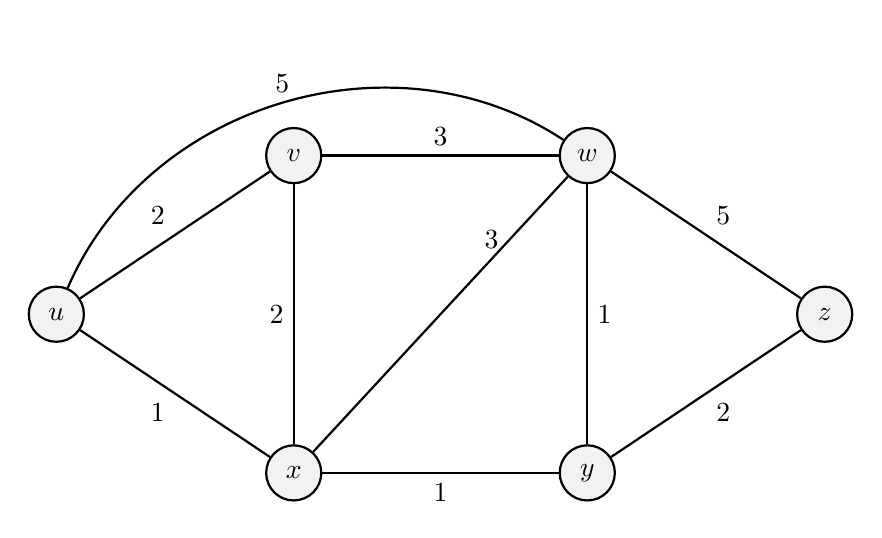
\begin{tikzpicture}[thick, main/.style = {draw, circle, minimum
      size=0.7cm, inner sep=0pt}]

      % --- Nodes ---
      \node[main, fill=gray!10] (u) {$u$};
      \node[main, fill=gray!10, above right=1.5cm and 2.5cm of u] (v) {$v$};
      \node[main, fill=gray!10, below right=1.5cm and 2.5cm of u] (x) {$x$};
      \node[main, fill=gray!10, right=3cm of v] (w) {$w$};
      \node[main, fill=gray!10, right=3cm of x] (y) {$y$};
      \node[main, fill=gray!10, below right=1.5cm and 2.5cm of w] (z) {$z$};

      % --- Edges (Using [-] to override the global ->) ---
      \path[-]
      (u) edge node[above left] {2} (v)
      (u) edge node[below left] {1} (x)
      (u) edge[bend left=50] node[above] {5} (w) % The curved top link

      (v) edge node[left] {2} (x)
      (v) edge node[above] {3} (w)

      (x) edge node[below] {1} (y)
      (x) edge node[pos=0.7, above] {3} (w) % Diagonal x-w

      (w) edge node[right] {1} (y)
      (w) edge node[above right] {5} (z)

      (y) edge node[below right] {2} (z);

    \end{tikzpicture}
  \end{figure}

  \begin{table}[H]
    \begin{center}
      \begin{tabularx}{\textwidth}{|X|X|X|X|X|X|X|}
        \hline
        step & $N'$ & $D(v)$,$p(v)$ & $D(x)$,$p(x)$ & $D(w)$,$p(w)$ &
        $D(y)$,$p(y)$ & $D(z)$,$p(z)$ \\
        \hline
        0  & $ \{u\}$ & 2, $u$ & 1, $u$ & 5, $u$ & $\infty$ & $\infty$ \\
        1 & $ \{u, x\} $ & 2, $u$ & & 4, $x$ & 2, $x$ & $\infty$ \\
        2 & $ \{u, x, y\} $ & 2, $u$ & & 3, $y$ &  &  4, $y$\\
        3 & $ \{u,x,y,v\} $ &  & & 3, $y$ &   & 4, $y$ \\
        4 & $ \{u,x,y,v,w\}$  & & & & & 4 $y$ \\
        5 & $ \{u,x,y,v,w,z\}$ & & & & & \\
        \hline
      \end{tabularx}
    \end{center}
  \end{table}

  \begin{enumerate}
    \item In the initialization step, we start with $N' = \{u\}$, and
      we set the initial distances to the neighbours of $u$:
      \begin{itemize}
        \item $D(v) = 2$, $p(v) = u$
        \item $D(x) = 1$, $p(x) = u$
        \item $D(w) = 5$, $p(w) = u$
        \item $D(y) = \infty$, $p(y) = -$
        \item $D(z) = \infty$, $p(z) = -$
      \end{itemize}
    \item In step 1, we add $x$ to $N'$ since, $D\left( x \right) =
      1$, i.e. the least cost neighbour, and  for all neighbours of
      $x \not\in  N'$:
      \begin{itemize}
        \item $w$ -  $D\left(x\right)_{1} + c \left( w, x \right)_{3}$ is
          less than $D\left( w \right)_{4} $, $D \left( w \right) = 4
          $, $p \left( w \right) = x $
        \item $v$ - $D\left( x \right)_1 + c \left( v, x \right)_2  $
          is not less than $D \left( v \right)_2 $, no change
        \item $y$ - $D \left( x \right)_1 + c \left( y, x \right)_1
          $ is less than $D \left( y \right)_{\infty} $, $D \left( y
          \right) = 2 $, $p \left( y \right) = x $
      \end{itemize}
      New state:
      \begin{itemize}
        \item $D(v) = 2$, $p(v) = u$
        \item $D(x) = 1$, $p(x) = u$
        \item $D(w) = 4$, $p(w) = x$
        \item $D(y) = 2$, $p(y) = x$
        \item $D(z) = \infty$, $p(z) = -$
      \end{itemize}
    \item In step 2, we add $y$ to $N'$ since, $D \left( y \right) =
      2 $, i.e. the least cost neighbour, and for all neighbours of
      $y \not\in N'$:
      \begin{itemize}
        \item $w$ - $D \left( y \right)_2 + c \left( y, w \right)_ 1
          $  is less than $D \left( w \right)_4 $, $D \left( w
          \right) = 3 $, $p \left( w \right) = y $
        \item $z$ - $D \left( y \right)_2 + c \left( y, z \right)_2
          $ is less than $D \left( z \right)_{\infty} $, $D \left( z
          \right) = 4 $, $p \left( z \right) = y $
      \end{itemize}
      New state:
      \begin{itemize}
        \item $D(v) = 2$, $p(v) = u$
        \item $D(x) = 1$, $p(x) = u$
        \item $D(w) = 3$, $p(w) = y$
        \item $D(y) = 2$, $p(y) = x$
        \item $D(z) = 4$, $p(z) = y$
      \end{itemize}
    \item And so on, we continue this process until all nodes are added to $N'$
      With the final state:
      \begin{itemize}
        \item $D(v) = 2$, $p(v) = u$
        \item $D(x) = 1$, $p(x) = u$
        \item $D(w) = 3$, $p(w) = y$
        \item $D(y) = 2$, $p(y) = x$
        \item $D(z) = 4$, $p(z) = y$
      \end{itemize}
  \end{enumerate}
}

When the LS algorithm terminates we have for each node it's
predecessor $p \left( v \right) $, along with the least-cost path
from the source node $u$ to $v$. The least-cost path can be
reconstructed by following the predecessor nodes from $v$ back to
$u$. The time complexity of Dijkstra's algorithm is $O \left( n^2
\right) $, where $n$ is the number of nodes in the graph. With the
use of a priority queue, the time complexity can be improved to $O
\left( m + n \log n \right) $, where $m$ is the number of edges in the graph.

\section{Distance Vector (DV) Routing}

The Distance Vector (DV) algorithm is iterative, asynchronous and
distributed. Each node receives some information from one or more of
its directly connected neighbours, computes the path, and then
distributes the results to its neighbours.

Le $d_x \left( y \right) $ be the cost of the least cost path from
node $x$ to $y$. Then the least costs are related by the Bellman-Ford equation:
\[
  d_x \left( y \right) = \min_v \left\{ c \left( x, v \right) + d_v
  \left( y \right)   \right\}
\]
Where the $\min_v$ is taken over all of $x$'s neighbours. This
equation states that after travelling from $x$ to $v$ if we take the
least cost path from $v$ to $y$, the path cost will be $c \left( x, v
\right)  + d_v \left( y \right) $, and since we must begin by
travelling to some neighbour $v$, the least cost from $x$ to $y$ is
the minimum of cost of $x$ to $y$ added to the least cost from $v$ to
$y$ taken over all neighbours $v$ of $x$.

For example given the earlier graph starting at node $u$, to
destination $z$, we have:
\begin{align*}
  d_u \left( z \right)  &=  \min \left\{ c \left( u, v \right) + d_v
    \left( z \right), c \left( u, w \right) + d_w \left( z \right), c
  \left( u, x \right) + d_x \left( z \right)   \right\}  \\
  \\
  d_v \left( z \right) &= \min \left\{ c \left( v, w \right) + d_w
  \left( z \right), c \left( v, x \right) + d_x \left( z \right)   \right\}   \\
  d_w \left( z \right) &=  5 \\
  d_x \left( z \right) &= \min \left\{ c \left( x, y \right) + d_y
  \left( z \right), c \left( x, w \right) + 5   \right\}   \\
  d_y \left( z \right)  &= 2 \\
  d_x \left( z \right) &= \min \left\{ 1 + 2, 3 + 5   \right\}   \\
  d_x \left( z \right) &= 3 \\
  d_v \left( z \right) &= \min \left\{ 3 + 5, 2 + 3   \right\}   \\
  d_v \left( z \right) &= 5 \\
  \\
  d_u \left( z \right)  &=  \min \left\{ 2 + 5, 5 + 5, 1 + 3   \right\}  \\
  d_u \left( z \right)  &= 4
\end{align*}

Each node $x$ begins with $D_x \left( y \right) $, an estimate of the
cost of the least cost pat from itself to $y$, or all nodes $y$ in $N$ let
\[
  \mbold{D_x} = \left\{ D_x \left( y \right) : y \in N \right\}
\]
be the distance vector, which is the vector of cost estimates from
$x$ to all other nodes, $y$ in $N$. With the DV algorithm, each node
$x$ maintains the following information:
\begin{itemize}
  \item For each neighbour $v$, the cost $c \left( x, v \right) $
    from $x$ to directly attached neighbour $v$.
  \item Node $x$'s distance vector $\mbold{D}_x$ containing $x$'s
    current estimate of its cost to all destinations $y$ in $N$.
  \item The distance vectors of each of its neighbours, that is
    $\mbold{D}_v$ for each neighbour $v$ of $x$.
\end{itemize}

When a node $x$ receives a new distance vector from any of its
neighbours, $w$ it updates its distance vector $\mbold{D}_x$ using
the Bellman-Ford equation:
\begin{align*}
  D_x \left( y \right) &=  \min_v \left\{ c \left( x, v \right) + D_v
  \left( y \right)   \right\} \text{for each node $y$ $N$}  \\
\end{align*}

If node $x$'s distance vector has changed as a result of then update,
the $x$ will send its updated distance vector to all its neighbours.
Eventually, if the network topology and link costs remain unchanged
for a sufficient amount of time, the distance vectors will converge
to the least cost paths from each node to all other nodes in the network.

\begin{algorithm}[H]
  \caption{Distance Vector (DV) Algorithm}
  \Comment{}\\
  \Comment{At each node $x$} \\
  \begin{algorithmic}[1]
    \State \textbf{Initialization:}
    \For{ all destinations $y$ in $N$}
    \State $D_x \left( y \right) = c \left( x, y \right) $
    \For{ each neighbour $w$}
    \State $D_w \left( y \right) = $ ? for all destinations $y$ in $N$
    \EndFor
    \For{ each neighbour $w$}
    \State send distance vector $\mbold{D}_x = \left\{ D_x \left( y
    \right) : y \in N \right\} $ to neighbour $w$
    \EndFor
    \EndFor
    \State
    \While{true}
    \State wait until a link cost change to some neighbour $w$ or
    until a distance vector $\mbold{D}_w$ is received from neighbour $w$
    \For{each $y$ in $N$}
    \State $D_x \left( y \right) = \min_v \left\{ c \left( x, v
    \right) + D_v \left( y \right)   \right\}  $
    \EndFor
    \If{$D_x \left( y \right) $ has changed for any destination $y$ in $N$}
    \For{ each neighbour $w$}
    \State send distance vector $\mbold{D}_x = \left\{ D _x \left( y
    \right) : y \in N \right\} $ to neighbour $w$
    \EndFor
    \EndIf
    \EndWhile
  \end{algorithmic}
\end{algorithm}

A node $x$ updates its distance-vector estimate when it either sees a
cost change in one of its adjacent nodes or receives a distance
vector from one of its neighbours. But to update its own forwarding
table for a given destination $y$, node $x$ needs to know the
neighbouring node $v*\left( y \right) $ that is the next hop router
along the shortest pat to $y$. The next hop router $v*\left( y
\right) $ is the neighbour $v$ that achieves the minimum in the
Bellman-Ford equation, i.e.

\subsection{Link-Cost Changes and Link Failure}

\subsection{Poisoned Reverse}

\section{Link State vs. Distance Vector}

\begin{description}
  \item[Message Complexity]  -
    \begin{description}
      \item[LS]  - Requires each node to know the cost of each link
        in the network, this requires $O \left(  \mid N \mid  \mid E
        \mid  \right) $ messages to be sent, also whenever a link
        cost changes the new link cost must be sent to all nodes.
      \item[DV] - Requires message exchanges directly between
        connected neighbours at each iteration, the time taken to
        converge depends on many factors such as the network
        topology, link costs, and the initial distance vector
        estimates. In general, DV can take a long time to converge,
        especially in large networks with many nodes and links.
    \end{description}
  \item[Convergence Speed]-
    \begin{description}
      \item[LS]  - Converges in $O \left(  \mid N \mid ^2 \right) $
        requiring $O \left(  \mid N \mid  \mid E \mid  \right) $ messages.
      \item[DV] - Convergence can be slow, especially in large
        networks, and can be affected by factors such as network
        topology and link costs. In some cases, DV can take a long
        time to converge, especially in large networks with many
        nodes and links. Also suffers from the count-to-infinity
        problem, where nodes can end up with incorrect distance
        estimates that keep increasing indefinitely.
    \end{description}
  \item[Robustness]-
    \begin{description}
      \item[LS]  - A router failure means that cost transmission may
        be incorrect for one of its attached links, a node could also
        corrupt or drop any packets it received as part of an LS
        broadcast, but an LS node is computing only its own
        forwarding tables, other nodes are not affected by a single
        node's failure, and the LS algorithm will continue to
        function correctly as long as the remaining nodes can
        communicate with each other.
      \item[DV] - A router failure can lead to a node advertising
        incorrect least-cost paths to any or all destinations,
        generally at each iteration a node's calculation in DV is
        passed on to its neighbour and then indirectly to it's
        neighbour's neighbour and so on causing an incorrect
        least-cost path to be advertised to all nodes in the network,
        this can lead to the count-to-infinity problem
    \end{description}
\end{description}

\chapter{Intra-Autonomous System (AS) Routing: Open Shortest Path
First (OSPF)}

The model of homogeneous routing within a network is not sufficient
for the Internet and fails in two areas:
\begin{description}
  \item[Scale] - As the number of routers becomes large the overhead
    involved in communicating computing, and storing routing
    information becomes prohibitive, and the time taken to converge
    can be very long.
  \item[Administrative Autonomy] - The Internet is a network of ISPs,
    with each ISP consisting of its own network or routers. An ISP
    generally desires to operate its network as it pleases and may
    not want to share information about its network topology and link
    costs with other ISPs. This is because of the competitive nature
    of ISPs, and the fact that sharing such information could
    potentially give competitors an advantage.
\end{description}

These problems can be solved by grouping routers into
\textbf{Autonomous Systems (AS)}, with each AS consisting of a group
of routers that are under the same administrative control. Each AS
can then use its own routing algorithm to determine the best path for
data to travel within its own network, while using a different
routing algorithm to determine the best path for data to travel
between ASes (lol). The routing algorithm running within an
autonomous system is called an \textbf{intra-AS routing Protocol}

\section{Open Shortest Path First (OSPF)}

OSPF is a widely used intra-AS routing protocol that is based on the
link-state routing algorithm. OSPF allows routers within an AS to
exchange information about the network topology and link costs,
enabling them to compute the least-cost paths to all destinations
within the AS. OSPF uses a hierarchical design, where the AS is
divided into areas, and each area has its own link-state database.

With OSPF each router constructs a complete topological map of the
network, and locally runs Dijkstra's algorithm to determine a
shortest path tree to all subnets, with itself as the root node.
Individual link costs are configured by the network administrator,
and can be based on various metrics such as bandwidth, delay, or
monetary cost. OSPF also supports features such as load balancing,
route summarization, and authentication to enhance the performance
and security of the routing protocol.

\chapter{Internet Service Provider (ISP) Routing: Border Gateway
Protocol (BGP)}

\section{The Role of BGP}

\section{Advertising BGP Route Information}

\section{Determining the Best Routes}

\subsection{Hot Potato Routing}

\subsection{Route Selection Algorithm}

\section{IP-Anycast}

\section{Routing Policy}

\section{Obtaining Internet Presence}

\end{document}
